\subsection{LMS vs. closed Form}
We followed the instructions and used the  function below with $G = 6$ to determine our $y$ values for the experimental setup.
\begin{equation}
f(x) = 2x^2 - Gx +1
\end{equation}


\begin{figure}[!h]
\begin{center}
\centering
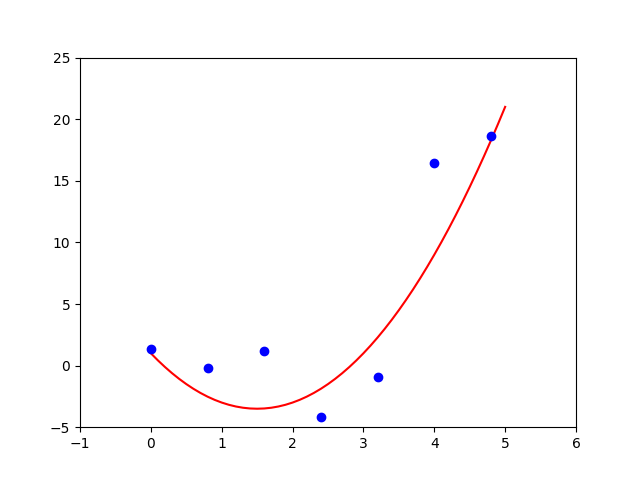
\includegraphics[width=5cm]{setup.png}
\end{center}
\caption{ Setup and an example of $t_i$ values with additional noise}
\end{figure}

\subsubsection{What is the resulting weight Vector when using the LMS rule?}

We implemented an online LMS learning rule for regression to determine useful weights to fit the curve. Figure \ref{ig:lms} shows three runs with randomised training data. As we can see the fitted curve is moved towards the original curve with each iteration. $\gamma$ or the learning factor controls how much impact new values have on the resulting weights for the next iteration. 

\begin{figure}[!h]
\begin{center}
\centering
\subfigure[]{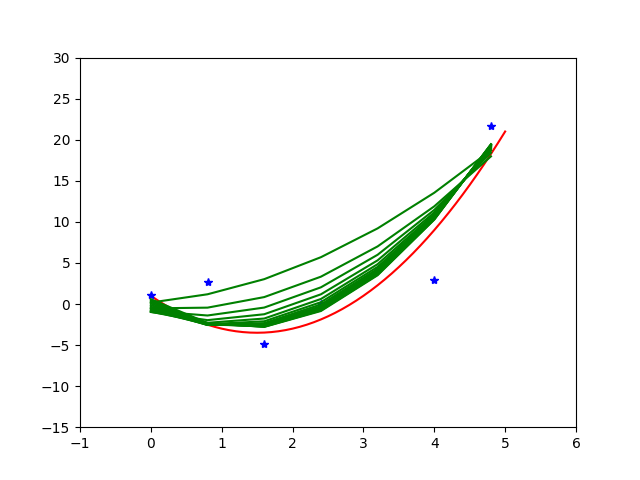
\includegraphics[width=5cm]{fig_lms_1.png}}
\subfigure[]{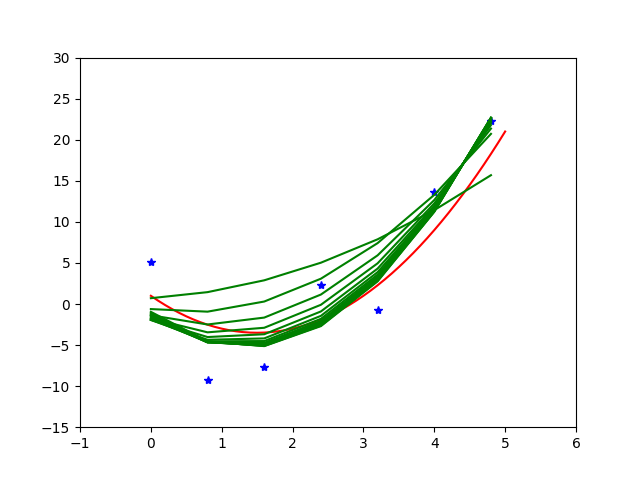
\includegraphics[width=5cm]{fig_lms_2.png}}
\subfigure[]{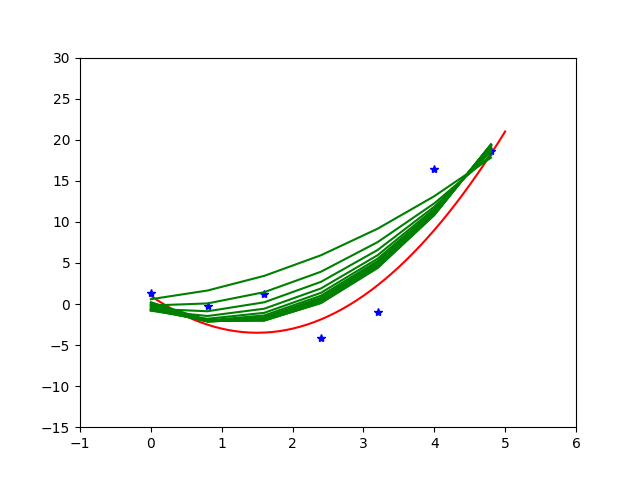
\includegraphics[width=5cm]{fig_lms_3.png}}
\subfigure[]{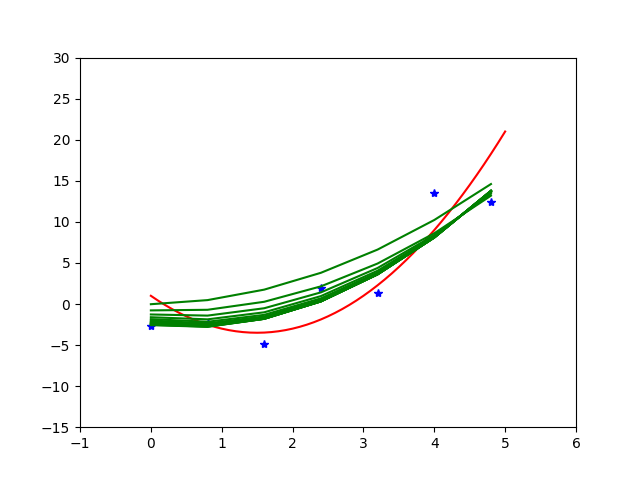
\includegraphics[width=5cm]{fig_lms_4.png}}
\end{center}
\caption{\label{fig:lms} Visualization of the learning process of \textbf{LMS}}
\end{figure}



\subsubsection{How can you determine the optimal $w*$ in closed form?  Compare $w*$ with the outcome of the {LMS}-rule training}

We used the pseudo inverse approach to minify the sum of squares error. As displayed the in the Tables, \ref{tab:error} and \ref{tab:weights} we can see the resulting weights and the calculated errors. We can see that the error rate for our four examples with CF are all better without much surprise.


\begin{figure}[!h]
\begin{center}
\centering
\subfigure[]{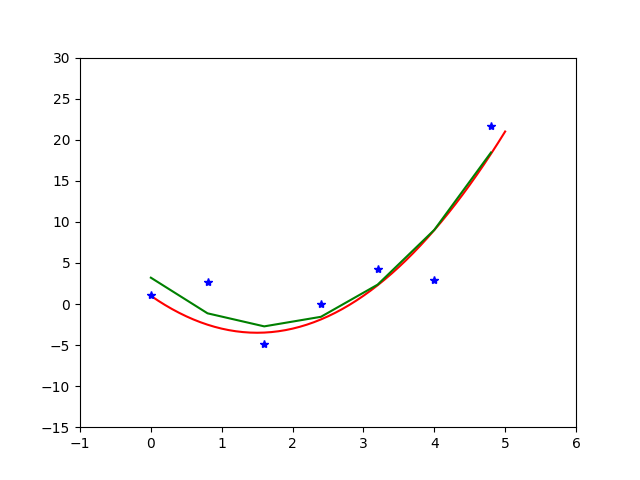
\includegraphics[width=5cm]{fig_cf_1.png}}
\subfigure[]{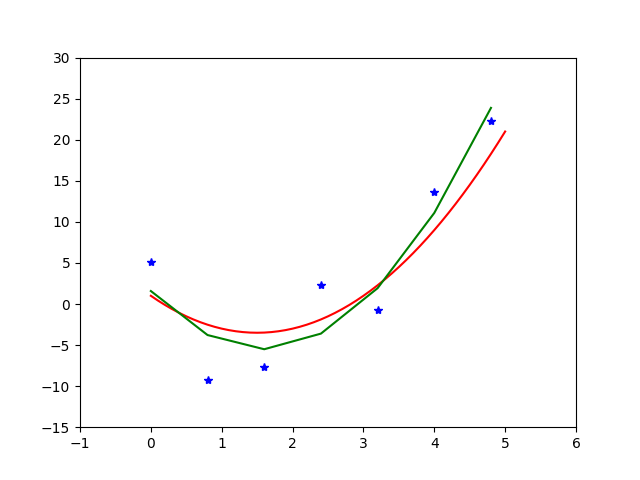
\includegraphics[width=5cm]{fig_cf_2.png}}
\subfigure[]{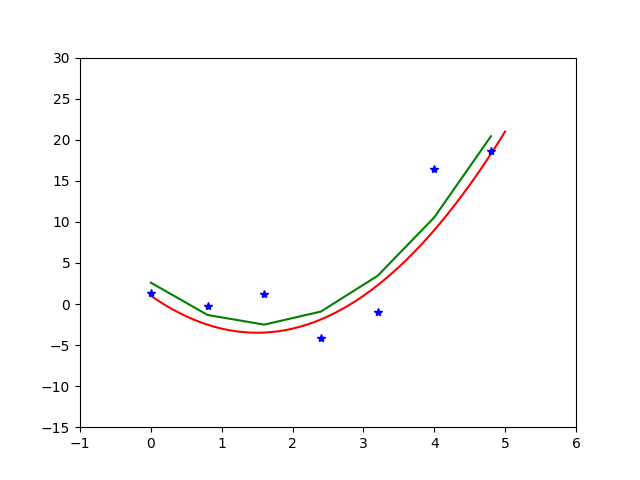
\includegraphics[width=5cm]{fig_cf_3.png}}
\subfigure[]{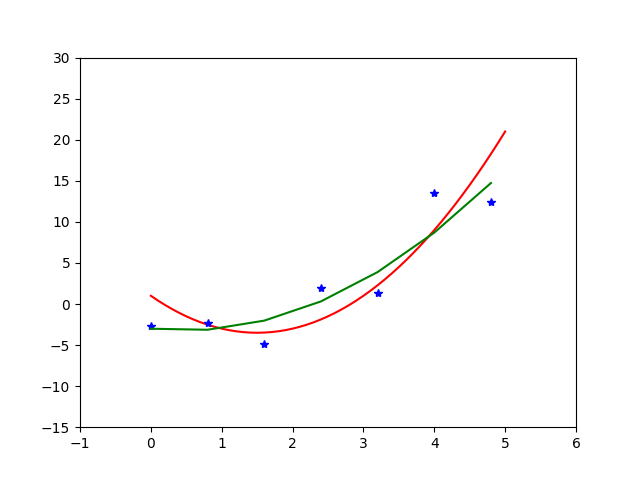
\includegraphics[width=5cm]{fig_cf_4.png}}
\end{center}
\caption{\label{fig:cf}the same training data as in figure, however this time solved in closed form (\textbf{CF}) }
\end{figure}



\begin{table}[!h]
\begin{tabular}{lll}
\textbf{Figure} & \textbf{LMS} & \textbf{CF} \\
a               &       97.09004286828198       &     71.03243449830224       \\
b               &      112.43543529868002        &     97.82006516766448          \\
c               &        109.4839763954856      &        84.46023189949588         \\
d               &        61.164485036889054      &         47.10797373501289        \\
\end{tabular}
\caption{\label{tab:error} error comparisons between{LMS} and {CF}}
\end{table}

\begin{table}[]
\begin{tabular}{lll}
\textbf{Figure} & \textbf{LMS} & \textbf{CF} \\
a               &        2.79641366 -4.06370085  1.6057828       &     6.10503808 -6.93083294  2.04038233       \\
b               &      0.90857717 -6.42409915  2.36363687        &     1.57854501 -8.9662967   2.8358482          \\
c               &        0.25694124 -4.13859362  1.69469808      &        2.59983553 -6.64808401  2.1588638         \\
d               &        -2.58665078 -0.97237072  0.9121616       &         -3.01226058 -0.92406774  0.96261322        \\
\end{tabular}
\caption{\label{tab:weights}resulting weights{LMS} and {CF}}
\end{table}


\subsubsection{Influence of $\gamma$ }

As mentioned earlier $\gamma$ has to influence if the algorithm can converge. In case $gamma$ is too big, new values get too much weight, thus 'overriding' older ones. See Figure \ref {fig:gamma}

\begin{figure}[!h]
\begin{center}
\centering
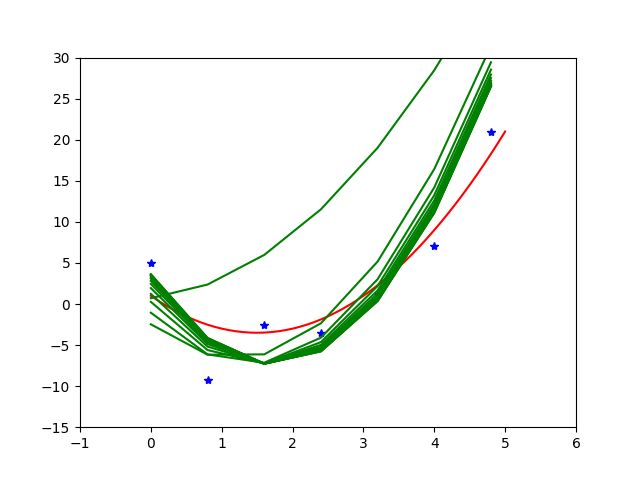
\includegraphics[width=5cm]{fig_gamma.png}
\end{center}
\caption{\label{fig:gamma} $\gamma$ has been chosen too high }
\end{figure}




\subsection{Image Data}
Unfortnuately we did not finish in time 
